\chapter{Molecular Dynamics}\label{ch:md}
Using the lessons learned in the previous chapter and after a reasonably successful validation of simulations (see section \ref{sec:sim_validation}), we can use the computational parameters at a lower precision and perform Molecular Dynamics simulations in VASP. The purpose of this chapter is to discuss the computational details, outline the chosen defect structures and finally present how defects (interstitial or otherwise) modifies the structure and dynamics of the parent compound. While molecular dynamics simulations are unable to provide information about the phonon band structure directly, it is possible to extract the phonon DOS and other relevant dynamical information as outlined in section \ref{sec:method_md}. In order to distinguish the simulations, we use a similar notation as in the previous chapter, but with the option to add dopants: [HTT/LTO/LTT][m]+[Sr/O$_\text{i}$], where omitting the [m] refers to the AFM electronic structure. For example, LTOm+Sr refers to a calculation starting from orthorhombic (Bmab) symmetry, in the metallic phase, with added Sr dopant.

\section{Computational Details}
Since Molecular Dynamics simulations require a large number of SCF cycles, it is necessary to drastically reduce the precision of our simulation. In general, the most drastic approximation comes from only running the simulation at one $k$-point ($\Gamma$). Other parameters are benchmarked by small test runs of a couple hundred steps and then evaluating the computational resources/time available. In our case we end up with the following additional reductions in precision:

\begin{itemize}
	\item Planewave cut-off at the default: \SI{400}{\eV} (\texttt{ENCUT=400})
	\item Threshold for the SCF to stop reduced to \SI{e-5}{\eV} (\texttt{EDIFF=1E-5})
	\item A faster algorithm for electronic minimization (\texttt{ALGO=F})
	\item Projection operators calculated in real space (\texttt{LREAL=A})
\end{itemize}

We keep the \texttt{PREC} tag set to `Accurate', since changing to `Normal' resulted in convergence issues. In addition, we need to specify the temperature and type of ensemble (see section \ref{sec:method_md}). For all simulations, we run at $T=\SI{300}{\kelvin}$ (\texttt{TEBEG=300}) within the canonical (NVT) ensemble using the algorithm of Nos\'{e} with a Nos\'{e}-mass such that the temperature fluctuates with a frequency of roughly \SI{38}{\tera\hertz} (\texttt{SMASS=1}). In order to get reasonable statistics we run with a time step $\Delta t = \SI{2}{\femto\second}$ (\texttt{POTIM=2}) for a total of 21000 (\texttt{NSW=21000}) steps, corresponding to a simulation time of \SI{42}{\pico\second}. For the analysis, we discard the first \SI{2}{\pico\second} in order to let the system equilibrate.

For the initial structures where defects have been added, we perform a geometry optimization of the supercell in order to find a structural minimum from which to start the MD simulation. Due to the reduced symmetry (compared to the phonon calculations in chapter \ref{ch:simulation}) this is a fairly expensive computation, so we perform the optimization with the same parameters as the MD simulation, except that we increase the $k$-point mesh to $4 \times 4 \times 4$ and the SCF threshold to \SI{e-6}{\eV}. Similar to the phonon calculations, we use the conjugate gradient algorithm for this minimization.

\section{Octahedral tilts}\label{sec:md_tilts}
\begin{figure}
	\centering
	\begin{subfigure}{0.64\textwidth}
		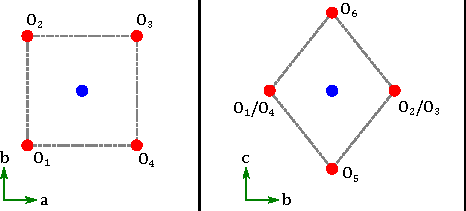
\includegraphics[width=\textwidth]{fig/md/q1q2_md_tilts.pdf}
	\end{subfigure}
	\begin{subfigure}{0.35\textwidth}
		\begin{align*}
			Q_1^1 &= \sin ^{-1} \left( \frac{O_6^x}{O_6^z} \right) \\
			Q_1^2 &= \sin ^{-1} \left( \frac{O_5^x}{O_5^z} \right) \\
			Q_1^3 &= \sin ^{-1} \left( \frac{O_1^z}{2 O_1^x} + \frac{O_2^z}{2 O_2^x} \right) \\
			Q_1^4 &= \sin ^{-1} \left( \frac{O_3^z}{2 O_3^x} + \frac{O_4^z}{2 O_4^x} \right)
		\end{align*}
	\end{subfigure}	
	\caption[Finding octahedral tilts from arbitrary oxygen positions]{Finding octahedral tilts from arbitrary oxygen positions. $Q_2$ angles can be found in an analogous way by replacing $x$ with $y$ and `pairing up' O$_1$ with O$_4$ and O$_2$ with O$_3$.}
	\label{fig:md_octahedral_tilts}
\end{figure}

In order to obtain octahedral tilts from MD simulations where symmetry is turned off, we are forced to define the octahedral tilts for each octahedra in the supercell. In fact, by writing which octahedra each oxygen atom (excluding interstitials) in our simulation belongs to, we can extract the $(Q_1,Q_2)$ tilt as seen from that oxygen. Since the tilts alternate, each tilt belongs to one of four symmetries with respect to $(Q_1,Q_2)$: (+,+), (+,-), (-,+), (-,-). In practice, we analyse the initial $t=0$ structure with the following steps for each Cu atom in the supercell:

\begin{enumerate}
	\item Record the position of the Cu atom
	\item Find apical oxygens by searching for (Cu, O) pairs with a distance less than $r = (1,1,2.7) \, \SI{}{\angstrom}$
	\item Find equatorial oxygens by searching for (Cu, O) pairs with a distance less than $r = (2.1,2.1,1) \, \SI{}{\angstrom}$
	\item Determine the $Q_1$, $Q_2$ tilt as seen from each of the 6 oxygen atoms in the list.
	\item Apply the symmetry operations.
	\item Save the 4 ($Q_1$, $Q_2$) value pairs.
\end{enumerate}

\noindent Step 4 is performed by first converting fractional coordinates to real-space coordinates and then finding angles as outlined in Figure \ref{fig:md_octahedral_tilts}. The symmetry operations in step 5 is a matrix with 8 columns corresponding to the 8 tilt values and a number of rows equal to the number of octahedra -- 16 in the case of our $2 \times 2 \times 1$ supercell. Each element of the matrix is either +1 or -1, where -1 will reverse the tilt direction and +1 will keep it as-is. The matrix can be generated by examining the output of the starting structure (which has the correct space group symmetry) and then constructing the matrix such that all $(Q_1, Q_2)$ tilts agree. While the same result can be archived by manually assigning the different atoms of our manageable supercell, this methodology allows the code to eventually be expanded to other systems, since we can set up arbitrary local coordinate systems.

After having performed this analysis, we can apply the same operations to every time step and obtain statistics about the time-evolution of the octahedral tilts in our system. This is similar to the Positional Recurrence Maps (PRM) methodology \cite{Piovano2016} that has been used to extract information about the apical oxygen dynamics in Nd$_2$NiO$_{4+\delta}$ \cite{Perrichon2015}.

\section{Structures with dopant ions}
Since the introduction of dopant ions breaks the crystal symmetry, we cannot perform phonon calculations using the direct method without making an excessive amount of high-precision calculations. Our typical $2 \times 2 \times 1$ supercell containing 112 ions with P1 symmetry would require $112 \times 3 = 336$ displacements just to describe phonon frequencies and eigenvectors at $\Gamma$. The worst case phonon calculation (LTT with magnetism) in the preceding chapter required just 21 displacements. For this reason, we are essentially forced to use molecular dynamics. In the following, the model for placing the initial dopants is outlined for Sr- and O-doped systems separately.

\subsection{LCO+O}
We start by considering the La$_2$CuO$_{4+\delta}$ System, which is simply LCO with added oxygen atoms at interstitial sites. It is generally accepted that the oxygen enters in the middle of the rock-salt layer, the least dense area of the crystal structure. Figure \ref{fig:oint_location} shows possible interstitial positions for the LTO (Bmab) and LTT (P4$_2$/ncm) phase, taken from a model proposed for the La$_2$NiO$_{4+\delta}$ system \cite{Tranquada1994}. Simulations in the defect phases are denoted by subscript `defect'. We ignore the HTT phase for molecular dynamics since the symmetry is broken and the preliminary geometry optimization would tend to tilt the octahedra similar to the LTT phase. To represent a reasonable doping level, we consider the addition of a single interstitial. It is generally accepted that the oxidation state is, at least approximately, O$^{2-}$, such that each dopant adds two holes. In our $2 \times 2 \times 1$ supercell with 16 formula units, this corresponds to a doping of $n_\text{h} = \frac{2}{16} = 0.125$.

\begin{figure}
    \centering
    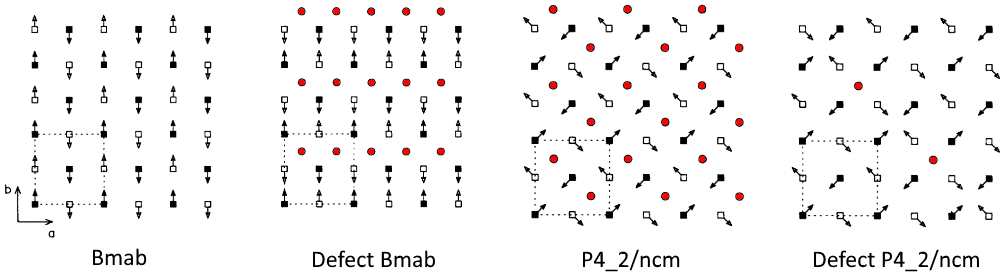
\includegraphics[width=\textwidth]{fig/md/oint.png}
    \caption[Illustration of interstitial positions]{Illustration of interstitial oxygen in-plane ($a$-$b$) location with respect to the apical oxygen displacements in the rock-salt layer. Open squares represent apical oxygens `hanging down' while closed squares represent apical oxygens `sticking up'. Interstitial oxygen are red circles and are shown on every possible interstitial site for clarity. Adapted from ref. \cite{Tranquada1994}.}
    \label{fig:oint_location}
\end{figure}

To see how the symmetry is broken, Table \ref{tab:oint_locations} shows the resulting space groups when inserting an interstitial into various starting symmetries. As expected, the symmetry is lowered substantially, especially if the $z$-component of the interstitial is different from $\frac{1}{4}$. While the symmetry isn't reduced to P1, it is difficult to imagine that any of the space groups in Table \ref{tab:oint_locations} could be used solve the observed superstructures in LCO+O (see section \ref{sec:lscoo}). Diffraction studies point to the interstitial being placed at either $\left(\frac{1}{4} \frac{1}{4} z \right)$ with $z$ close to $\frac{1}{4}$ or on a general $(xyz)$ position \cite{Rial1997}. When modelling this position in diffraction studies, it is possible to keep the parent symmetry by assigning an occupation factor to the interstitial and thus keeping the symmetry of the parent phase. Since we are not afforded that luxury when building structures for molecular dynamics, defects will naturally break the symmetry of our parent phase. Table \ref{tab:oint_locations} should thus not be seen as proposed models, but rather as an illustration of our inability to model partial occupancies in a small real-space box.

\begin{table}
	\centering
	\caption[Oxygen interstitial phases]{Space group symmetry due to the introduction of an interstitial oxygen in various structures all described in a $2 \times 2 \times 1$ supercell of the Bmab (conventional) coordinate system. HTT, LTO and LTT are the usual phases as described in literature \cite{Hucker2012}. The structures labelled defect is (1) in the LTO case: A stacking fault where the middle layer has its tilts reversed and (2) in the LTT case: A line along [110] with reversed tilts. Both are described in \cite{Tranquada1994} and are designed in order to `make room' for the interstitial oxygen (see Figure \ref{fig:oint_location}).}
    \label{tab:oint_locations}
    \begin{tabular}{@{}lllll@{}}
\toprule
Phase                   & Space Group & $\text{O}_\text{i}^x$ & $\text{O}_\text{i}^y$ & $\text{O}_\text{i}^z$ \\ \midrule
HTT                     & I4/mmm (139)      &         &         &         \\
HTT + O$_\text{i}$      & P-42m  (111)    & 0.125   & 0.125   & 0.25    \\
HTT + O$_\text{i}$      & Cmm2 (35)       & 0.125   & 0.125   & 0.24    \\
LTO                     & Bmab (64)       &         &         &         \\
LTO + O$_\text{i}$      & P2 (3)    & 0.125   & 0.125   & 0.25    \\
LTO + O$_\text{i}$      & P2 (3)         & 0.125   & 0.125   & 0.24    \\
LTO$_\text{defect}$     & Pmna (53)       &         &         &         \\
LTO$_\text{defect}$ + O$_\text{i}$ & P2 (3)         & 0.875   & 0.375   & 0.25    \\
LTO$_\text{defect}$ + O$_\text{i}$ & P2 (3)         & 0.875   & 0.375   & 0.24    \\
LTT                     & P4$_2$/ncm (138)  &         &         &         \\
LTT + O$_\text{i}$      & P-4 (81)        & 0.375   & 0.125   & 0.25    \\
LTT + O$_\text{i}$      & P2 (3)         & 0.375   & 0.125   & 0.24    \\
LTT$_\text{defect}$               & Pmma (51)       &         &         &         \\
LTT$_\text{defect}$ + O$_\text{i}$ & Cmm2 (35)       & 0.875   & 0.375   & 0.25    \\
LTT$_\text{defect}$ + O$_\text{i}$ & Cmm2 (35)       & 0.875   & 0.375   & 0.24    \\ \bottomrule
\end{tabular}

\end{table}

\subsection{LSCO}
In the La$_{2-x}$Sr$_x$CuO$_4$ system, our current best guess is that the distribution of the doped Sr species is completely random and homogeneous. Since randomness is difficult to implement in a (relatively) small system with periodic boundary conditions, we initially place them at a distance of about half the box side in order to  represent homogeneous doping. Replacing La$^{3+}$ with Sr$^{2+}$ adds one hole, so we add two dopants in order to be at $n_\text{h} = 0.125$ doping.

\section{Geometry Optimization}
We performed high-precision geometry optimizations of ionic positions only on these LCO+O defect structures starting from the various relevant symmetries. The starting structures were the optimized structures from chapter \ref{ch:simulation} with an interstitial inserted according to Table \ref{tab:oint_locations}. The defect structures were created by reversing certain tilts according to Figure \ref{fig:oint_location}. For the geometry optimization we kept the volume fixed at the value obtained from the parent structures without tilt defects, substitutions or interstitials. Performing an equation-of-state geometry optimization for all structures as in section \ref{sec:sim_geomopt} is computationally expensive for the defect supercells, but Figure \ref{fig:lcoo_eos} shows a EOS fit of the LTT structure with a limited number of points, revealing that the Volume does not change significantly due to the interstitial.

\begin{figure}
	\centering
	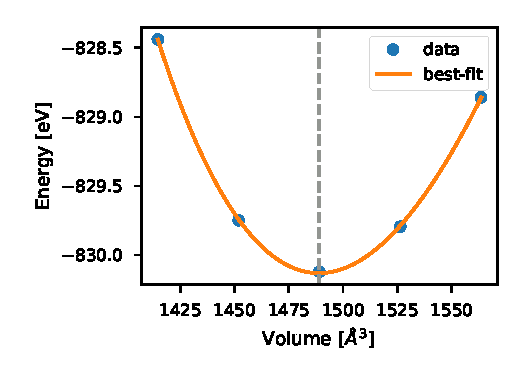
\includegraphics[width=0.6\textwidth]{fig/md/lcoo_eos.pdf}
	\caption[LCOO EOS]{Equation-of-state fit to La$_2$CuO$_{4.0625}$ starting from the LTT phase with one added interstitial oxygen in our supercell. The broken vertical line is the minimum of the fit, showing that our starting volume was reasonable. Each minimization was performed without symmetry while relaxing both ionic positions and the cell shape. The orthorhombic strain due to the cell shape change was below $\eta = 0.0004$ for all volumes, suggesting that the tetragonal crystal shape is a stable minimum.}
	\label{fig:lcoo_eos}
\end{figure}

Table \ref{tab:oint_lcoo_en} shows the resulting total energies and ($Q_1, Q_2$) tilts for a variety of starting structures including oxygen interstitials. A few trends emerge from this investigation. First, the defect structures in Figure \ref{fig:oint_location} has the effect of reducing the \emph{average} tilt of the structure, if we keep the symmetry operations from the non-defective phase. In the case of LTO the average tilts completely cancel out, while in the case of LTT they are cut in half. In addition, both the average and local tilts move towards the tilt pattern of the non-defective phase during optimization. In general, our simulations find that it costs more energy to reverse the tilts compared to the addition of the interstitial. This is inconsistent with the observation of staging (see section \ref{sec:lscoo}) and is likely related to the limited size of our simulation. Since a well-defined energy minimum is important for the initial configuration of the MD simulations, we stick with the parent, undistorted phases when investigating LCO+O. Finally, we notice that the tilts tend towards an `LTT-like' tilt-pattern in the optimization of metallic LTO, while keeping a significant orthorhombic strain. 

\begin{table}[b]
	\centering
	\caption[Oxygen interstitial phases: Energy]{Oxygen interstitial phases, geometry optimization. Geometry optimization performed on ionic positions only. $E_0$ corresponds to the energy after inserting the interstitial oxygen, but before geometry optimization. $E_1$ is the total energy after optimization. The octahedral tilts ($Q_1, Q_2$) are similarly defined before and after the optimization.}
	\label{tab:oint_lcoo_en}
	\begin{tabular}{llllll}
    \toprule
	 & $E_0$ [eV] & $E_1$ [eV] & $(Q_1, Q_2)_0$ & $(Q_1, Q_2)_1$  \\ 
	\midrule
    HTT + O$_\text{i}$                    & -827.27669             & -829.76250 & (0.00, 0.00) & (1.00, 1.00) \\
    LTO + O$_\text{i}$                    & -828.29890             & -830.39658  & (0.00, 5.79) & (1.21, 5.92) \\
    LTO$_\text{defect}$ + O$_\text{i}$            & -823.09516             & -830.03588  & (0.00, 0.00) & (2.12, 4.48) \\
    LTT + O$_\text{i}$                    & -828.04663             & -830.08248  & (4.61, 4.61) & (3.77, 3.72) \\
	LTT$_\text{defect}$ + O$_\text{i}$             & -826.03173             & -829.94243  & (2.31, 2.31) & (2.80, 2.70) \\
	LTOm + O$_\text{i}$                & -872.73074             & -876.56079  & (0.00, 6.42) & (3.76, 3.90) \\
	LTTm + O$_\text{i}$                & -872.35546             & -876.56195  & (4.53, 4.53) & (3.85, 3.85) \\
	\bottomrule
    \end{tabular}
\end{table}

Table \ref{tab:oint_lsco_en} shows the same optimizations performed on Sr-doped La$_2$CuO$_4$. The results here are as we expect from the small difference between the ionic radius of La$^{3+}$ and Sr$^{2+}$ (see table \ref{tab:dopants}). We seem to be in a well-defined minimum and the average tilt is only modified slightly. While geometry optimizations are only able to locate a local minimum, the results in Tables \ref{tab:oint_lcoo_en} and \ref{tab:oint_lsco_en} point toward the expected conclusion that interstitial oxygen has a more significant effect on the octahedral tilt patterns compared to Sr doping. The nature of these effects cannot be obtained from geometry optimizations alone, and we turn to molecular dynamics for the detailed analysis of structure and dynamics.

\begin{table}[b]
	\centering
	\caption[Sr doped phases: Energy]{Sr doped phases, geometry optimization. $E_0$ corresponds to the energy after replacing La with Sr, but before geometry optimization. $E_1$ is the total energy after optimization. Geometry optimization performed on ionic positions only. The octahedral tilts are similarly defined before and after the optimization.}
	\label{tab:oint_lsco_en}
	\begin{tabular}{lllll}
    \toprule
	 & $E_0$ [eV] & $E_1$ [eV] & $(Q_1, Q_2)_0$ & $(Q_1, Q_2)_1$  \\ 
	\midrule
    LTO + Sr                  & -858.73485             & -859.48650  & (0.00, 5.79) & (0.00, 5.38) \\
	LTOm + Sr                    & -858.57712             & -859.39905  & (0.00, 6.42) & (0.00, 5.69) \\
	LTT + Sr                    & -858.68994            & -859.49712  & (4.61, 4.61) & (3.87, 3.97) \\
	LTTm + Sr                    & -858.57810           & -859.40170  & (4.53, 4.53) & (3.98, 4.08) \\
	\bottomrule
    \end{tabular}
\end{table}

\section{Benchmarking}
Similar to our phonon calculations in the previous chapter, molecular dynamics simulations are typically benchmarked in various ways. Depending on the type of ensemble and thermostat, either the temperature or total energy is expected to be conserved. It is, however, possible for numerical noise to cause these quantities to drift. In our case the Nos\'{e} thermostat controls temperature through velocities, so it can be useful to plot the temperature as a function of simulation time to see if the fluctuations are reasonable. The temperature can be calculated from the MD trajectory by first computing the velocities through the Verlet algorithm (see section \ref{sec:method_md}) and then evaluating
%
\[ T = \frac{1}{3 k_\text{B} (N_\text{ions}-1)} \sum_j M_j |\bm{v}_j|^2 \, , \]
%
where $N_\text{ions}$ is the number of atoms, $M_j$ is the mass of atom $n$ and $\bm{v}_j$ is the velocity of atom $j$. We divide by $(N_\text{ions} - 1)$ rather than $N_\text{ions}$, since temperature is defined with respect to degrees of freedom and we can arbitrarily redefine our coordinate system with respect to a particular atom. When considering the instantaneous temperature in this way, we expect the mean-squared temperature fluctuations to be \cite{Hickman2016}
%
\[ \left\langle \left( \Delta T^2 \right) \right\rangle = \frac{2T_0^2}{3N_\text{ions}} \, . \]
%
Four our simulation with $N_\text{ions} = 112$ at $T_0 = \SI{300}{\kelvin}$ we thus expect temperatures fluctuations of $\pm \SI{23.15}{\kelvin}$. Figure \ref{fig:stitch} is a summary of benchmarks performed on the LCO in the LTO phase with no dopant ions or defects. Simulations were performed with two different time steps and the difference in temperature fluctuations and the resulting phonon DOS was recorded. In terms of temperature fluctuations, there is little effect of going from 1 to 2 fs time steps, but there are slight modifications to the DOS, especially in the region around 30 meV. While this may be seen as problematic, it is important to realize that we are probing a relatively small number of steps, and it is unlikely that our simulation is completely ergodic. In other words, we may be probing a different area of phase space in the two simulations. It is unlikely that the time step resolution itself is causing the effects on DOS, since an energy of \SI{30}{\milli\eV} = \SI{7.3}{\tera\hertz} is probed by simulation times of roughly \SI{137}{\femto\second}. While higher precision is always desirable, we stick with a time step of \SI{2}{\femto\second} in order to be able to probe dynamics for longer time scales in more systems. Now, almost by definition, different time steps do probe different dynamics. I emphasize that any comparison between MD simulations is done at the same time step.

\begin{figure}
	\centering
	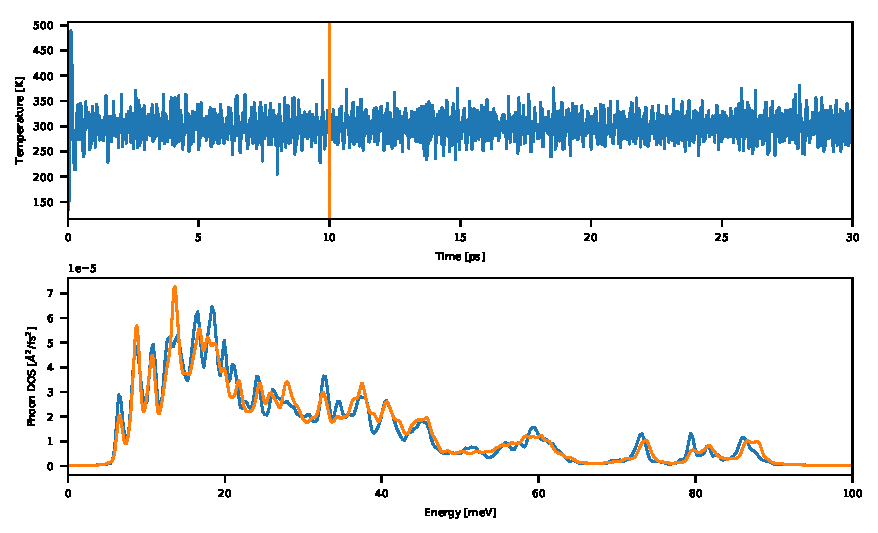
\includegraphics[width=\textwidth]{fig/md/stitch.pdf}
	\caption[stitched md runs]{Benchmark of molecular dynamics, using LCO in the LTO phase with no dopant ions or defects. \textbf{Top:} Temperature fluctuations for a simulation stitched together with the first \SI{10}{\pico\second} using a \SI{1}{\femto\second} time step and the last part of the simulation using a \SI{2}{\femto\second} time step. \textbf{Bottom:} Density of States weighted by neutron-cross sections and broadened by a Gaussian with $\sigma=\SI{0.5}{\milli\eV}$ (\SI{1.18}{\milli\eV} FWHM) evaluated at the same two parts of the simulation.}
	\label{fig:stitch}
\end{figure}

\section{DOS and PDF}
Molecular dynamics simulations have been performed with 7 starting configurations based on geometry optimizations in Table \ref{tab:oint_lcoo_en} and \ref{tab:oint_lsco_en} as well as references without dopant ions. Since the full matrix of combinations now includes 3 structural phases, 2 dopant ions, 2 electronic phases and 2 `defect' phases, the total number of desired simulations is 20. In order to limit the scope and focus computational resources, we chose to focus on the LTO phase and end up with the following list of simulations:

\begin{enumerate}
	\item LTT: LTT in AFM phase.
	\item LTO: LTO in AFM phase.
	\item LTO+Sr: LTO in AFM phase with added Sr dopants.
	\item LTO+O: LTO in AFM phase with added O dopant.
	\item LTOm: LTO in metallic phase.
	\item LTOm+Sr: LTO in metallic phase with added Sr dopants.
	\item LTOm+O: LTO in metallic phase with added O dopant
\end{enumerate}

Our primary observables when comparing to experiment is the phonon density of states and pair-density-function. We start by considering the DOS of all simulations, calculated with the method described in section \ref{sec:method_md} and the scripts developed in appendix \ref{app:software}. Figure \ref{fig:lto_md_defect_comparison} shows the neutron-weighted phonon DOS for all 7 simulations. While the overall shape of the phonon DOS is mostly unchanged, there are some subtleties that we might consider for further analysis. For the magnetic simulations, we see a similar modification of modes at $\approx \SI{30}{\milli\eV}$ when comparing the LTO and LTT phases. Interestingly, the sharp dip in DOS at \SI{30}{\milli\eV} is seen in LTO+O as well. In fact, the LTT and LTO+O phases appear to share more qualitative features with each other compared to the parent LTO phase. This is consistent with the initial geometry optimization of LCO+O in table \ref{tab:oint_lcoo_en} moving towards a LTT-like tilt pattern. LTO+Sr, on the other hand, mostly seem to broaden features rather than directly modify then. 

For the metallic simulations, we see similar trends but in a much more smeared out fashion, possibly due to reduced accuracy of these simulations due to the fermi surface smearing (see figure \ref{fig:sim_bench_para} in section \ref{sec:sim_benchmark}). Similar to the observations in chapter \ref{ch:simulation}, the main modification of the phonon DOS compared to the magnetic simulations is related to the high energy modes.

\begin{figure}
	\centering
	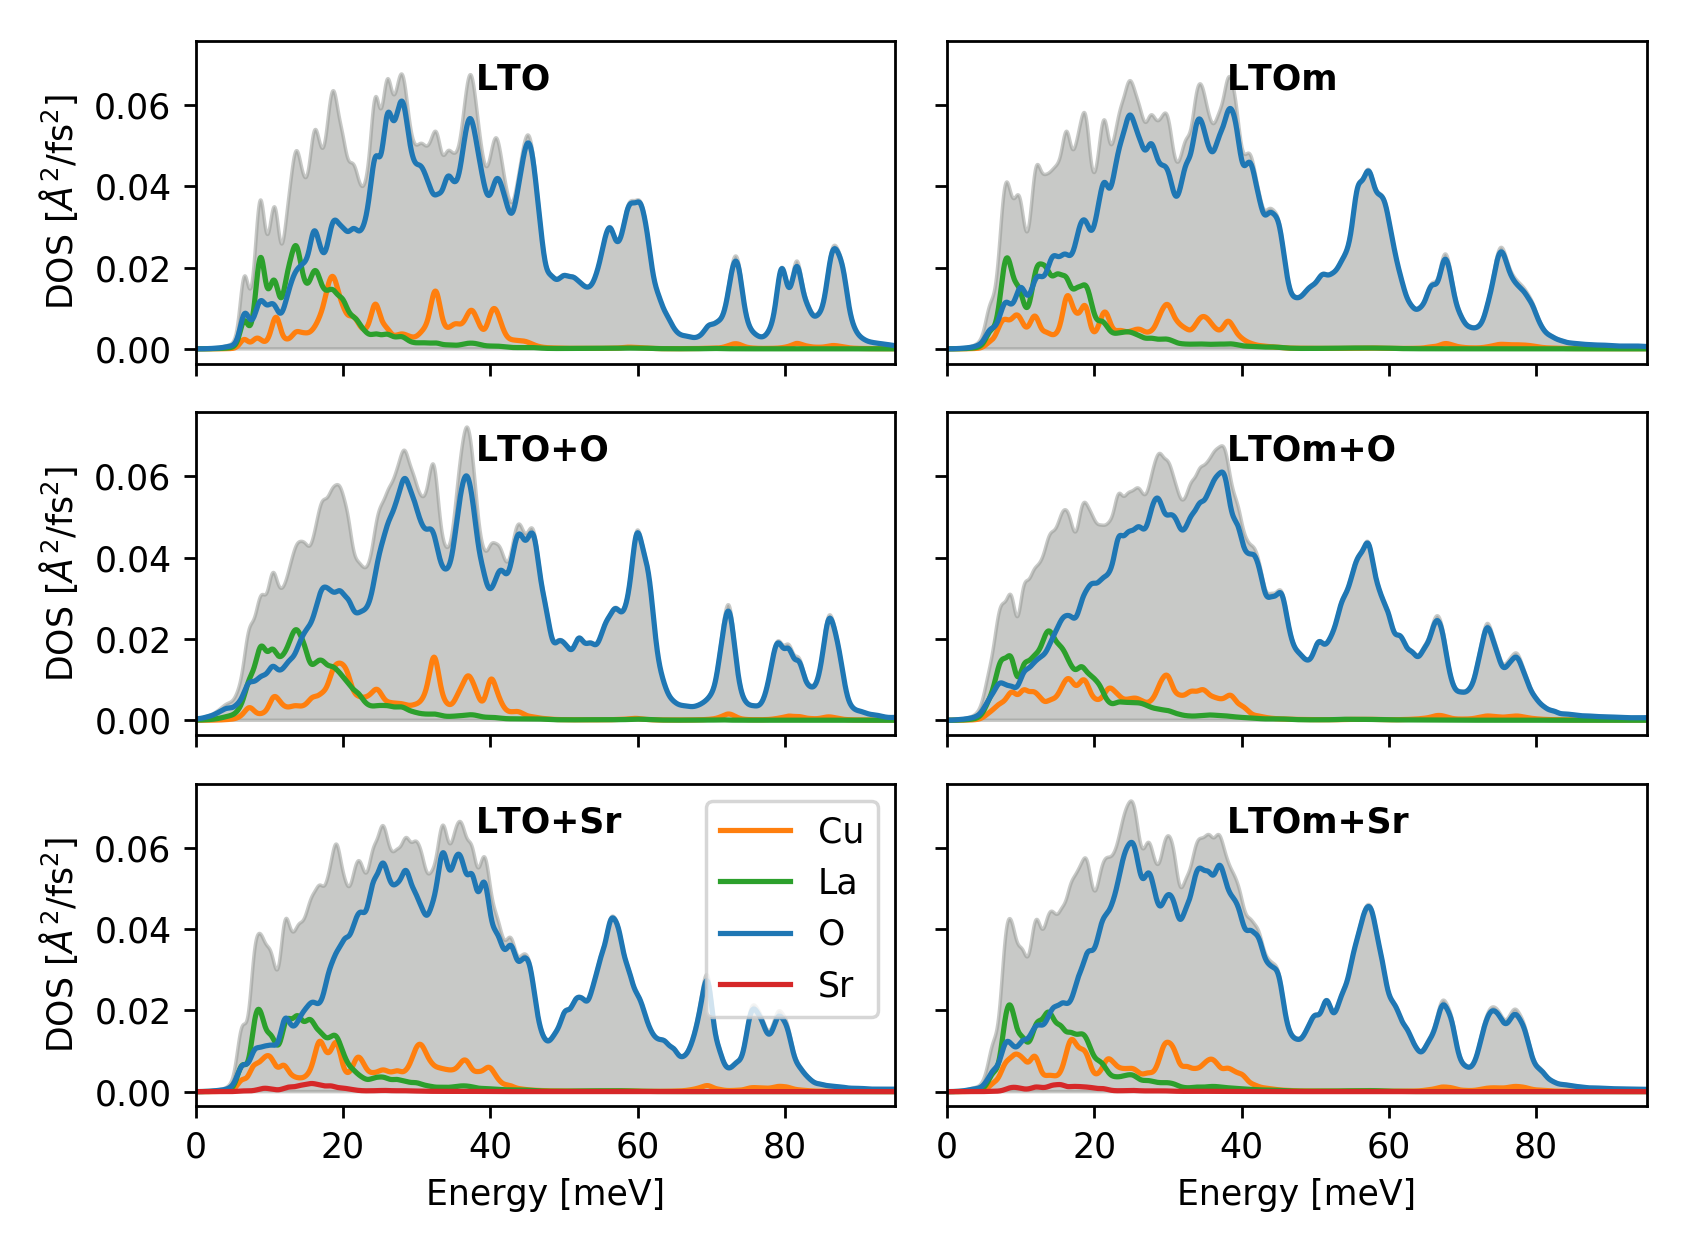
\includegraphics[width=\textwidth]{fig/md/lto_defect_comparison.png}
	\caption[LTO MD DOS: Defect comparison]{Neutron-weighed density-of-states for all molecular dynamics simulations performed in this chapter. The filled grey area is the total DOS and the lines are the partial atomic DOS. The initial conditions for the MD simulation is annotated on each plot according to the notation outlined in the beginning of this chapter. The density-of-states was obtained through the power spectrum of the velocity autocorrelation function (see section \ref{sec:method_md}). The power spectrum was smoothed by a Gaussian kernel with width $\sigma=\SI{0.5}{\milli\eV}$ (\SI{1.18}{\milli\eV} FWHM).}
	\label{fig:lto_md_defect_comparison}
\end{figure}

In order to compare more directly these observations, Figure \ref{fig:dos_pdf} shows a direct comparison of DOS and PDF of our LTO, LTO+O and LTT simulations. This comparison clearly shows that the LTT and LTO+O share common features especially around \SI{30}{\milli\eV} (various $c$-axis modes, see section \ref{sec:sim_dos} and \SI{60}{\milli\eV} (apical oxygen bond-stretching mode). The PDF in the same figure show only very subtle deviations, most notably around \SI{5.2}{\angstrom} where, once again, the LTT simulation shares features with LTO+O.

\begin{figure}
	\centering
	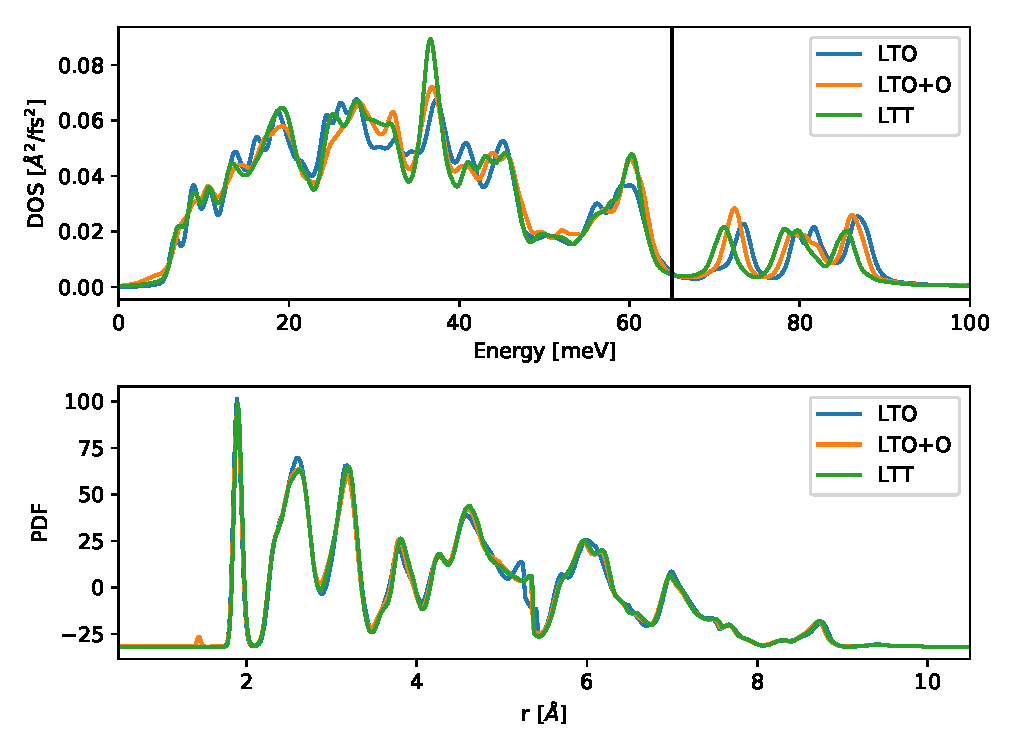
\includegraphics[width=\textwidth]{fig/md/lto_ltt_ltoo_comparison.pdf}
	\caption[MD: DOS and PDF]{\textbf{Top}: Total DOS for selected MD simulations. In general, differences are subtle, but we see some surprising similarities between the LTO+O and LTT simulation, indicating LTT-like behavior due to the interstitial (see text). \textbf{Bottom}: PDF of the same simulations, showing almost identical spectra for the 3 simulations. At roughly \SI{5.2}{\angstrom} there is a small modification where, once again, LTO+O and LTT simulations show similarities.}
	\label{fig:dos_pdf}
\end{figure}

\section{Microscopic analysis}
In addition to observables for comparison with experiment, the purpose of molecular dynamics simulations is to relate microscopic phenomena to these observables. For this reason, we will try to extract relevant information from the simulation trajectory in order to understand what is causing the changes in the phonon DOS and PDF. In the cuprates, there is much experimental evidence of the fact that Cu-O distances and distributions are important for superconductivity \cite{Bozin2000, Peng2017, Ivashko2019}. Inspired by these results, Figure \ref{fig:md_distances} show the distribution of Cu-O$_\text{equatorial}$ and Cu-O$_\text{apical}$ distances for selected simulations. In general, they follow a normal distribution showing that the harmonic approximation works well for our system, with the notable exception of the apical oxygen distance in LTO+O. 

\begin{figure}
	\centering
	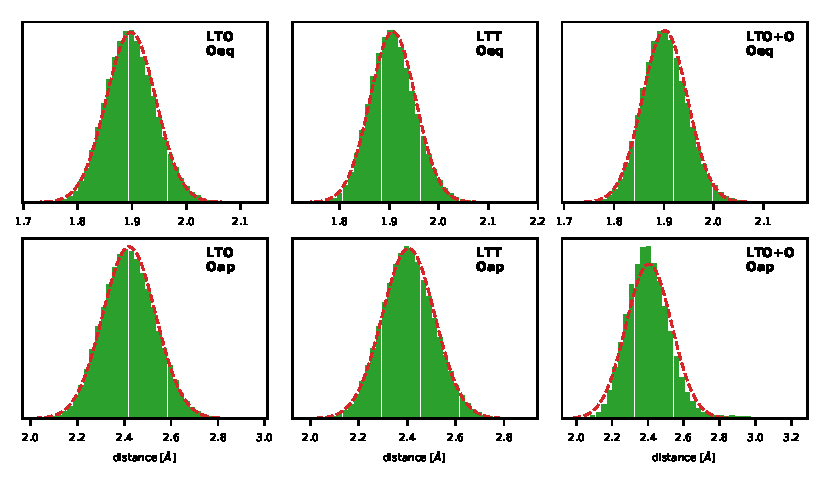
\includegraphics[width=\textwidth]{fig/md/dist_hist.pdf}
	\caption[MD: distance histograms]{Distance histograms of Cu-O distances with respect to the equatorial oxygen (Oeq) and apical oxygen (Oap) in the three simulations we compared in Figure \ref{fig:dos_pdf}. The data was generated by recording all appropriate distances at every time step of the simulation. The $y$-axis is normalized to unity and the broken line is a Gaussian function with expected value and variance calculated from the data. The histograms are normalized to unity.}
	\label{fig:md_distances}
\end{figure}

Table \ref{tab:md_cu_o_distances} summarizes these distances for all of the performed simulations. As expected from the almost identical PDF across simulations, the mean Cu-O$_\text{equatorial}$ distances does not seem to have any discernible trends, but there is a slight widening of the distributions in the systems containing dopants. In some sense this is expected since we have created different local environments by the introduction of impurity dopants. The same trend can be seen in the Cu-O$_\text{apical}$ distanced, but here we additionally have an shortening of the mean distance due to the introduction of oxygen (notice also that this shortening is identical to the LTT distance in magnetic case). For Sr-doping there is an elongation in the magnetic simulation but a shortening in the metallic simulation. It is, however, important to note that these differences are extremely subtle and may just be due to numerical peculiarities.

\begin{table}
	\centering
	\caption{Cu-O Distances distance statistics for all MD simulations performed in this chapter. Columns 2 and 3 show the mean distance and standard deviation for the Cu-O equatorial distance. Column 3 is the $R^2$ value of a linear regression assuming a normal distribution. Columns 4-6 show the same values for the Cu-O apical distance.}
	\label{tab:md_cu_o_distances}
	\begin{tabular}{lllllll}
		\toprule
			name &   $\langle \text{O}_\text{eq} \rangle $ [\AA]  & $\sigma$ (O$_\text{eq}$) [\AA] &  $R^2$ (O$_\text{eq}$) & $ \langle \text{O}_\text{ap} \rangle$ [\AA] & $\sigma$ (O$_\text{ap}$) [\AA] &  $R^2$ (O$_\text{ap}$) \\
		\midrule
			 LTO &  1.898 &  0.0455 &  0.9972 &  2.421 &   0.113 &  0.9989 \\
		   LTO+O &  1.902 &  0.0464 &  0.9972 &  2.406 &   0.127 &  0.9608 \\
		  LTO+Sr &  1.898 &  0.0507 &  0.9947 &  2.438 &   0.146 &  0.9995 \\
			LTOm &  1.909 &  0.0514 &  0.9951 &  2.462 &   0.140 &  0.9997 \\
		  LTOm+O &  1.908 &  0.0532 &  0.9934 &  2.440 &   0.156 &  0.9992 \\
		 LTOm+Sr &  1.905 &  0.0523 &  0.9947 &  2.451 &   0.151 &  0.9992 \\
			 LTT &  1.907 &  0.0461 &  0.9971 &  2.406 &   0.109 &  0.9992 \\
		\bottomrule
		\end{tabular}
\end{table}

Using the definitions of octahedral tilts described in section \ref{sec:md_tilts}, Figure \ref{fig:md_q1_q2_all} shows a histogram of $(Q_1, Q_2)$ tilts from all of our performed MD simulations on a logarithmic scale. Similar to observations from DOS and PDF, the tilt patterns of LTO+O are LTT-like, while the Sr-doped and parent compounds have tilts distributed around $(Q_1, Q_2) = (0,5)$ which is the equilibrium LTO structure. We also notice that the LTT-like simulations (LTT, LTO+O, LTOm+O) are able to transition between the  symmetrically equivalent tilt patterns, while the LTO-like simulations are `stuck' in the initial configuration. This is an indication that LTT-like tilts have distinct dynamics compared to LTO-like tilts.

\begin{figure}
	\centering
	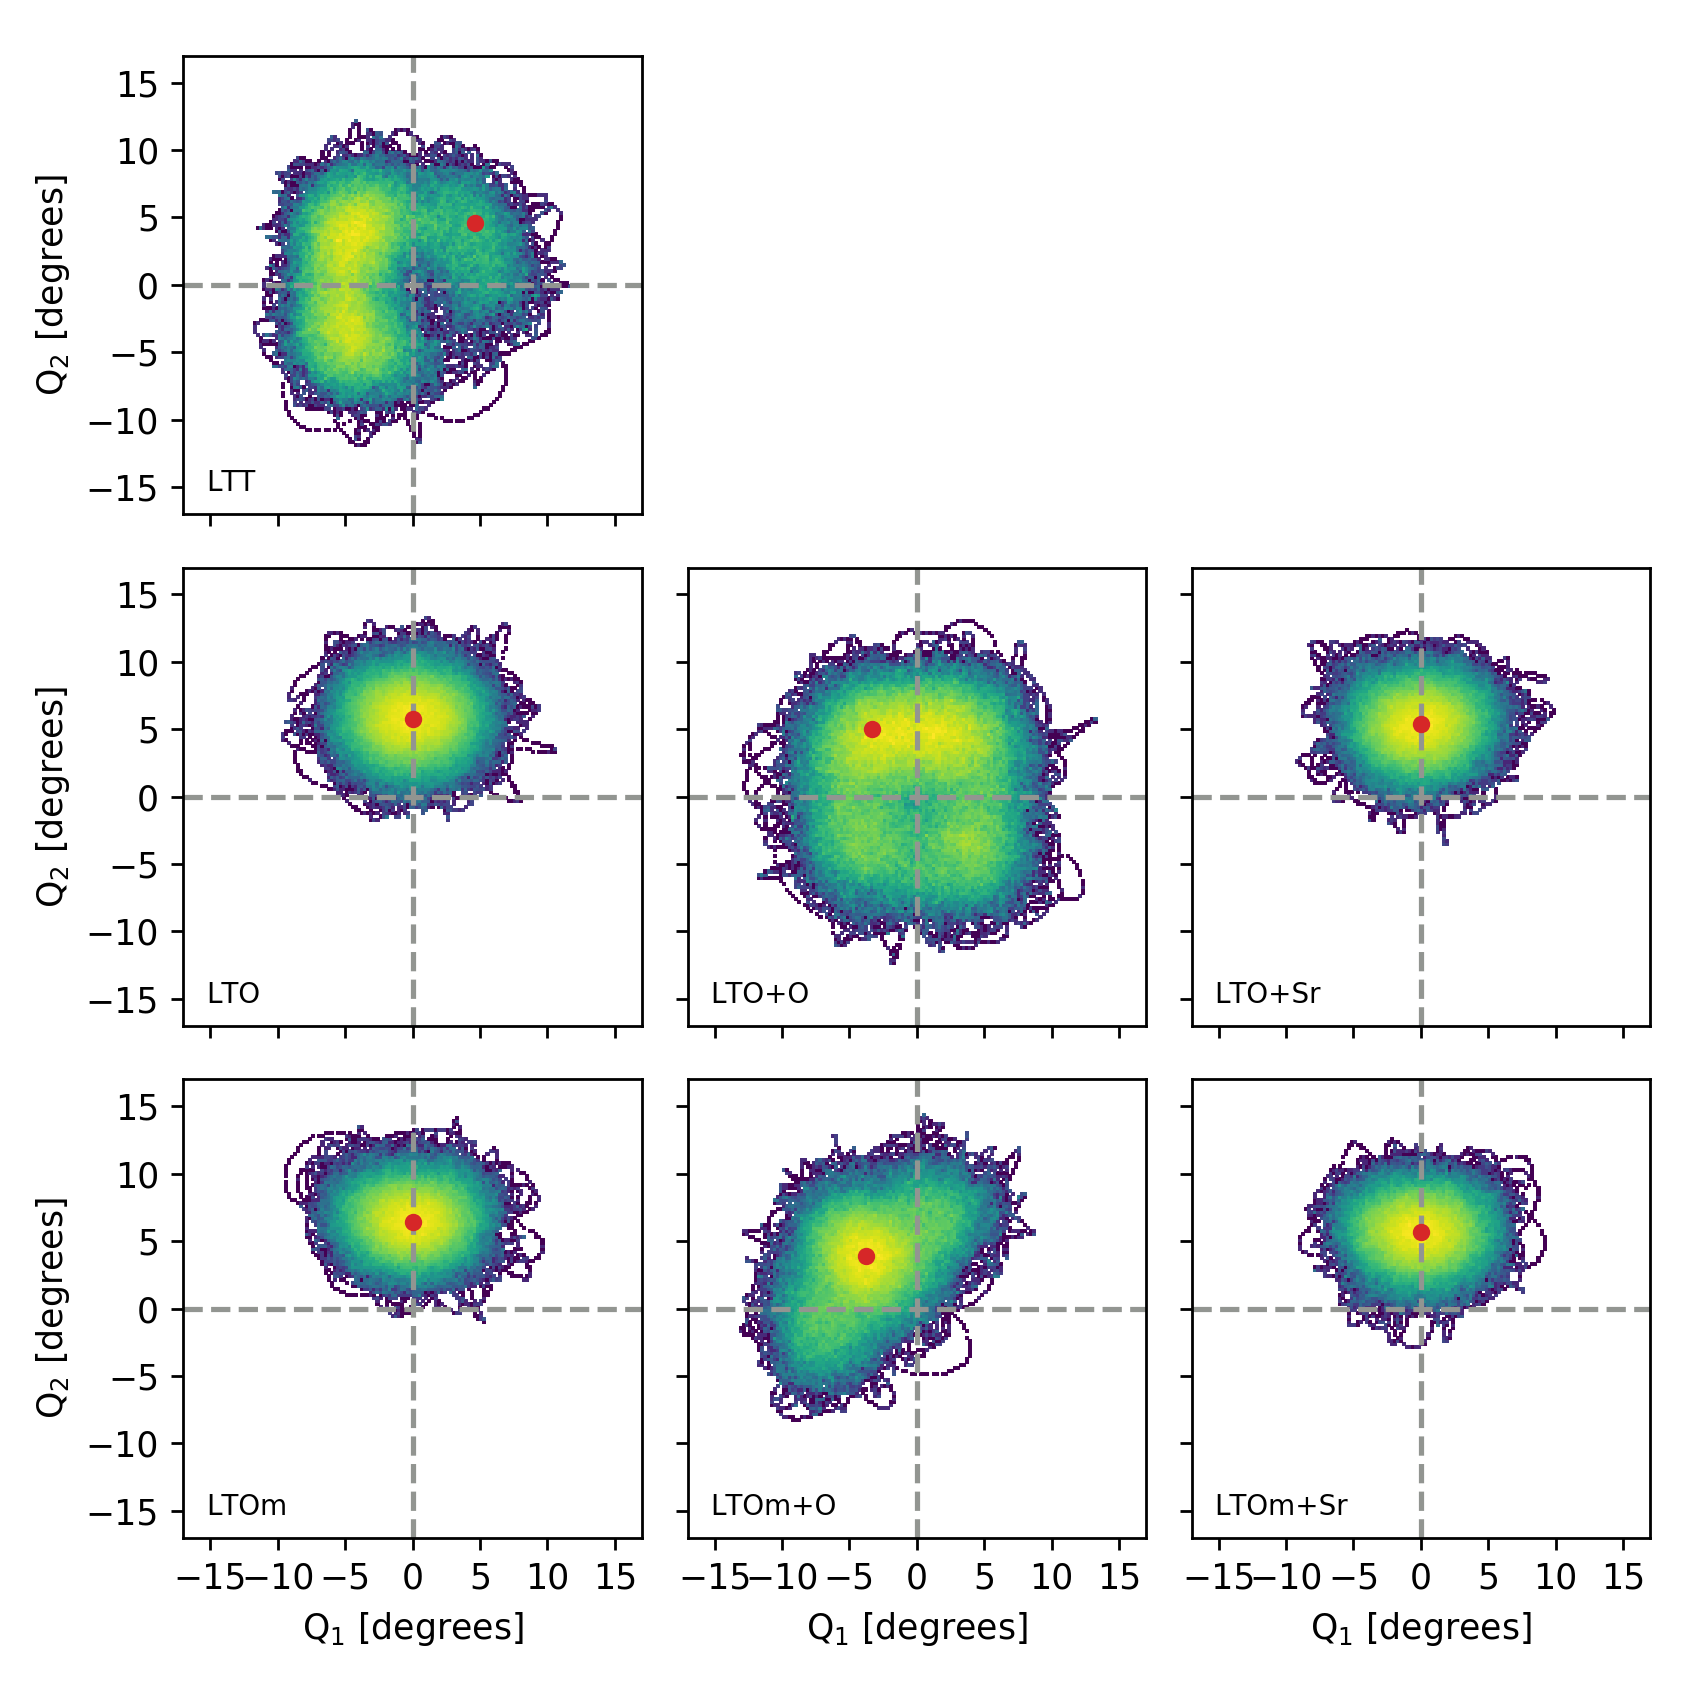
\includegraphics[width=\textwidth]{fig/md/Q1_Q2_all.png}
	\caption[MD Q1 Q2 All sims]{Tilt histograms of all performed molecular dynamics simulations. Plots are generated by obtaining the tilt as seen from apical oxygens and pairs of equatorial oxygens (as described in section \ref{sec:md_tilts}) for each time step and then plotting a 2D histogram of the resulting data on a logarithmic scale. The red circle denotes the starting tilt. As discussed in the text, we distinguish between LTT-like tilts sitting on the diagonals of this figure and LTO-like tilts sitting along the main axes. The same symmetry operations are applied at each time step, such that transitions between symmetrically equivalent configurations is visible in this plot.}
	\label{fig:md_q1_q2_all}
\end{figure}

Finally, figures \ref{fig:md_diffusion1} investigates the dynamics of the placed interstitial in LTO+O by following the in-plane location of the interstitial by plotting a histogram of its location as well as a line depicting its time evolution at equally spaced points in time. Additionally, we plot the $c$-axis evolution with a 1d histogram. For contrast, Figure \ref{fig:md_diffusion3} shows the same plots for a `normal' apical oxygen. Finally, Figure \ref{fig:md_diffusion2} shows the distribution of the apical oxygen near the interstitial, revealing a very similar distribution. These figures together show that the interstitial forms a `binary system' with the closest apical giving rise to a very localized effect. At $T=\SI{300}{\kelvin}$ we thus see no indication of diffusion. In some sense this is not surprising since diffusion is likely slow and not accessible within our relatively short \SI{40}{\pico\second} simulation times. In fact, the estimated `annealing time' for La$_2$CuO$_{4+\delta}$ has been estimated to be one week at room temperature \cite{Lee2004} (1 week divided by \SI{40}{\pico\second} is roughly $10^16$).

\begin{figure}
	\centering
	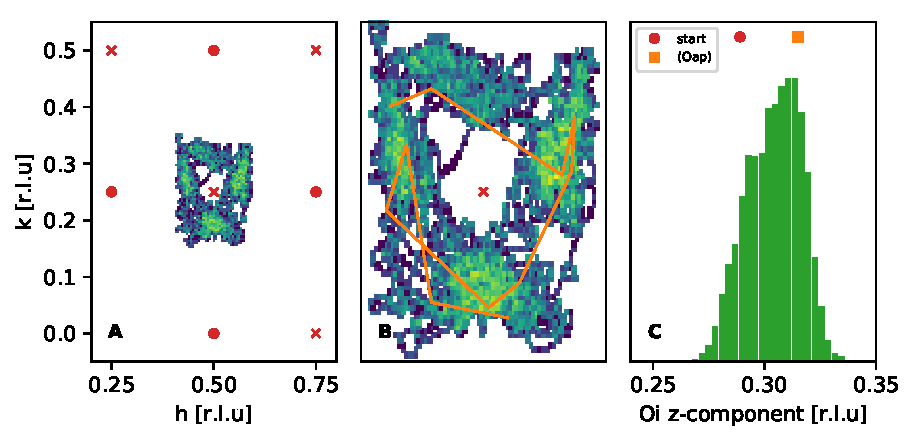
\includegraphics[width=\textwidth]{fig/md/diffusion1.pdf}
	\caption[MD Oint Diffusion Oi]{Distribution of the interstitial oxygen in LTO+O. \textbf{(A)}: In-plane distribution of the interstitial. Circles denote apical oxygens `sticking up', while crosses denote apical oxygen `hanging down' (similar to Figure \ref{fig:oint_location}). \textbf{(B)}: Zoomed-in version of \textbf{(A)} with the line marking the time-evolution of the interstitial sampled at isochronal points. \textbf{C}: $c$-coordinate distribution of the interstitial with the initial and average position marked in red and orange, respectively.}
	\label{fig:md_diffusion1}
\end{figure}

\begin{figure}
	\centering
	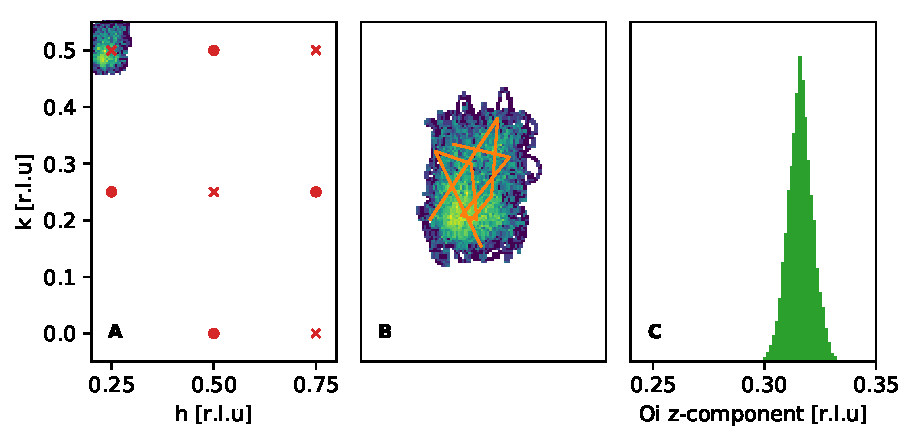
\includegraphics[width=\textwidth]{fig/md/diffusion3.pdf}
	\caption[MD Oint Diffusion Oap 2]{Distribution of a normal apical oxygen in LTO+O. \textbf{(A)}: In-plane distribution of the apical. Circles denote apical oxygens `sticking up', while crosses denote apical oxygen `hanging down' (similar to Figure \ref{fig:oint_location}). \textbf{(B)}: Zoomed-in version of \textbf{(A)} with the line marking the time-evolution of the interstitial sampled at isochronal points. \textbf{C}: $c$-coordinate distribution of the apical.}
	\label{fig:md_diffusion3}
\end{figure}

\begin{figure}
	\centering
	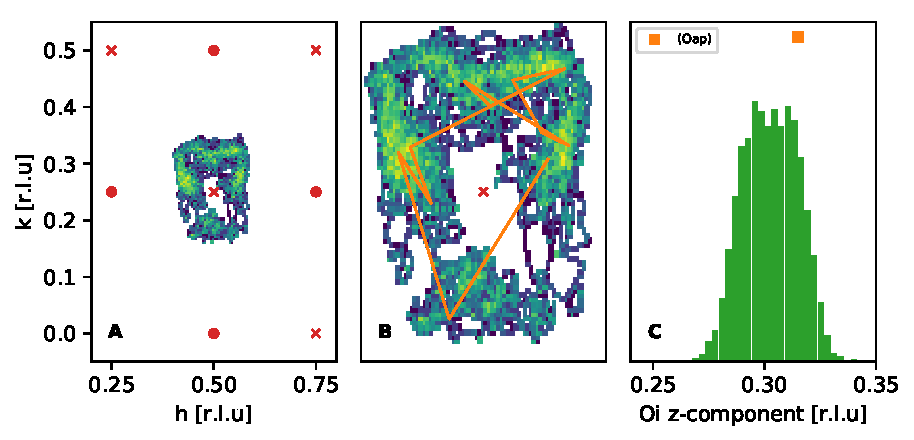
\includegraphics[width=\textwidth]{fig/md/diffusion2.pdf}
	\caption[MD Oint Diffusion Oap 1]{Distribution of an apical oxygen in LTO+O near the interstitial. \textbf{(A)}: In-plane distribution of the apical. Circles denote apical oxygens `sticking up', while crosses denote apical oxygen `hanging down' (similar to Figure \ref{fig:oint_location}). \textbf{(B)}: Zoomed-in version of \textbf{(A)} with the line marking the time-evolution of the interstitial sampled at isochronal points. \textbf{C}: $c$-coordinate distribution of the apical, with the average position marked in orange.}
	\label{fig:md_diffusion2}
\end{figure}

\section{Summary}
The main take-home message from chapter is the fact that interstitials seem to have a very subtle effect on structure but a more significant effect on dynamics. In particular, an observable such as PDF will se barely any difference between our simulations but high-quality DOS measurements should be able to see subtle differences due to dopants.

If we can obtain a reasonable validation of these simulations, the microscopic analysis reveals very clearly that oxygen interstitial phases move towards LTT-like tilt dynamics. Since the average structure of LCO+O at accessible temperatures is LTO, a possible explanation is that this tendency toward LTT-like tilts can result in the observed superstructures (and/or staging) \cite{Ray2017,Fratini2010} if we had access to bigger simulation boxes and longer simulation times. It might be valuable to examine this more closely with real-space methods such as reverse monte-carlo (RMC) or by performing classical MD based on the results obtained in this chapter.

Before moving on to experimental comparisons, Figure \ref{fig:md_phonopy_comparison} shows a comparison of phonon DOS as calculated from the previous chapter and the one obtained from molecular dynamics here. While there is a definite distinction between the spectra, it is important to realize that they are obtained by very different methods, while being based on the same computational background. In addition, molecular dynamics are not constrained by symmetry.

A direct comparison between molecular dynamics and phonon calculations should thus only be performed with extreme caution. For this reason, we mainly use the phonon calculations to identify the kinds of bands that correspond to certain features in the phonon DOS. When analyzing the role of dopants, simulations will all be done in the context of molecular dynamics (e.g. figure \ref{fig:dos_pdf}). In the experimental chapters I will leverage the phonon band structure calculations in context of triple-axis measurements of single crystals. Molecular dynamics simulations, on the other hand, will be used in the context of PDF and inelastic time-of-flight measurements of powdered samples.


\begin{figure}
	\centering
	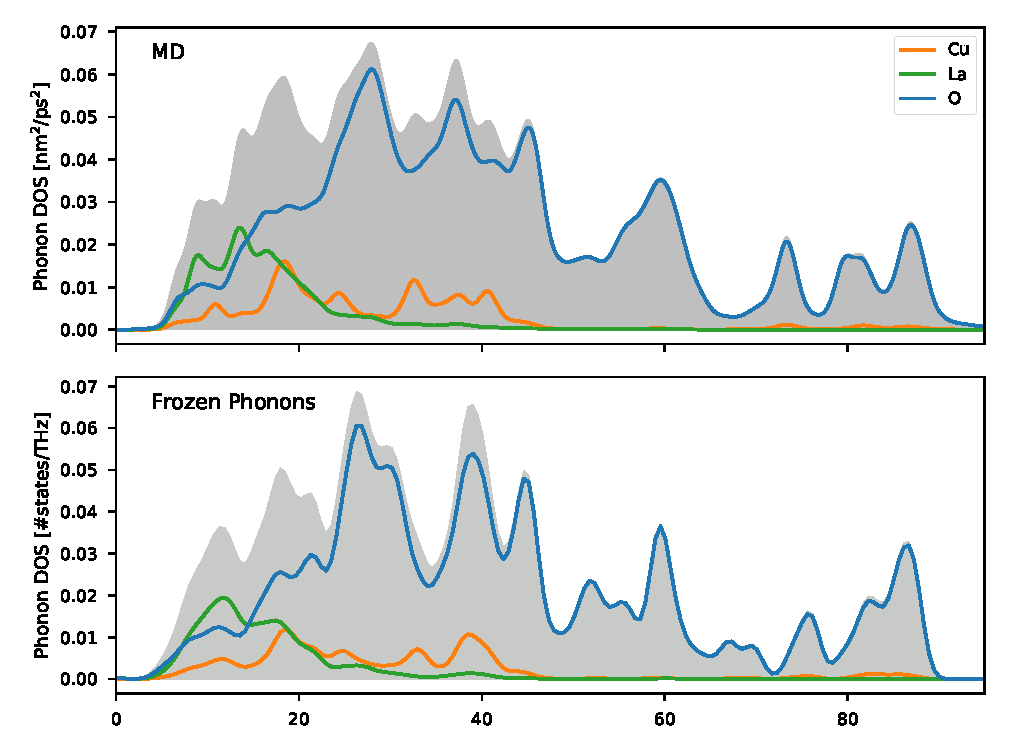
\includegraphics[width=\textwidth]{fig/md/md_phonopy_comparison.pdf}
	\caption[MD Phonopy Comparison]{Comparison of neutron-weighted phonon density of states obtained from \textbf{top:} the velocity autocorrelation function of a molecular dynamics trajectory and \textbf{bottom:} by integration of phonon bands calculated using the direct method (see chapter \ref{ch:simulation}). Both simulations are based on the low-temperature orthorhombic (LTO) structural phase.}
	\label{fig:md_phonopy_comparison}
\end{figure}


